\section{Description des connections}\label{sec:DescConnect}
L'ensemble des étages d'alimentation et de commande sont placés dans un boîtier électrique qui se branche sur une prise classique T13 230~V. Ce dernier
devra alimenter le contrôleur EPOS4 Compact 50/15 de chez Maxon \cite{Maxon} et la carte Raspberry Pi 3B+ \cite{RaspberryPi}. Une tension continue de 48~V
sera nécessaire pour commander le moteur et une tension continue de 5~V pour alimenter le Raspberry Pi. Pour obtenir ces tensions,
un convertisseur AC-DC avec 48~V en sortie et un convertisseur DC-DC avec 48~V en entrée et 5~V en sortie seront nécessaires. La fiche 230~V
sera une fiche pour appareil C14 avec bouton et fusible intégrés ce qui enlève la nécessité de mettre un disjoncteur et fait gagner de la place. Les deux
convertisseurs, le contrôleur et la carte de commande sont tous fixés sur un rail DIN35. Il faut donc déterminer les dimensions de ces éléments pour
déterminer la taille du boîtier et du rail nécessaire.\\

Le contrôleur est aussi connecté à l'encodeur linéaire et angulaire, à l'anneau de LEDs et aux capteurs de fin de course. On peut résumer toutes
ces connexions sur le schéma suivant.

\begin{figure}[H]
    \centering
    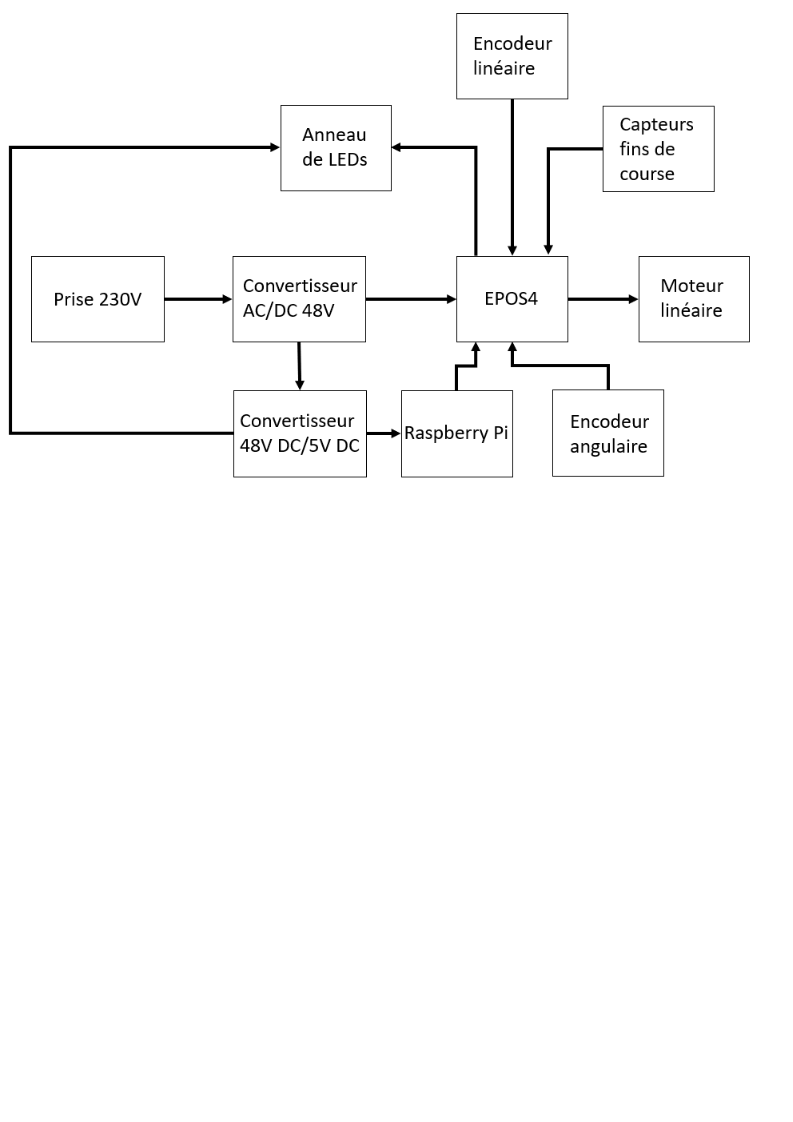
\includegraphics[width = 0.9\textwidth]{assets/figures/SchemaLogique.svg}
    \caption{Schéma de connexions}
    \label{fig:SchemaConnec}
\end{figure}

\section{Choix des éléments}\label{sec:ChoixElem}

\begin{table}[H]
    \centering
    \caption{Éléments choisis pour le boîtier électrique}
    \label{tab:ChoixElem}
    \resizebox{\textwidth}{!}{%
        \begin{tabular}{|l|l|l|l|l|l|}
            \hline
            Élément                       & Choix               & Fabricant                         & Hauteur {[}mm{]} & Largeur {[}mm{]} & Profondeur {[}mm{]} \\ \hline
            Convertisseur AC-DC 48V       & DRC100US48          & XP Power \cite{XPPower}           & 93               & 70               & 58                  \\ \hline
            Convertisseur DC-DC 48V-5V    & DDR-15L-5           & MEAN WELL \cite{MEANWELL}         & 90               & 17.5             & 54.5                \\ \hline
            Contrôleur moteur             & EPOS4 Compact 50/15 & Maxon \cite{Maxon}                & 65.5             & 59.5             & 35                  \\ \hline
            Carte de commande             & Raspberry Pi 4      & Raspberry Pi \cite{RaspberryPi}   & 85               & 56               & 30                  \\ \hline
            Connecteur fiche 230V         & C14                 & Schurter \cite{Schurter}          & -                & -                & -                   \\ \hline
            Bouton arrêt d'urgence        & AB6E-3BV02PTRH      & IDEC \cite{IDEC}                  & -                & -                & -                   \\ \hline
            Bouton poussoir               & 82-5151.1134.B001   & EAO \cite{EAO}                    & -                & -                & -                   \\ \hline
            Presse étoupe M8              & EX1100.08.035       & Agro \cite{Agro}                  & -                & -                & -                   \\ \hline
            Presse étoupe M10             & EX1100.10.040       & Agro \cite{Agro}                  & -                & -                & -                   \\ \hline
            Connecteur Moteur             & D-sub13W3           & Deltron Connectors \cite{Deltron} & -                & -                & -                   \\ \hline
            Connecteur Encodeur linéaire  & D-sub15             & -                                 & -                & -                & -                   \\ \hline
            Connecteur Encodeur angulaire & D-sub9              & -                                 & -                & -                & -                   \\ \hline
        \end{tabular}%
    }
\end{table}

La somme des largeurs des éléments est de 203~mm, la hauteur la plus grande est de 93~mm et la profondeur la plus élevée est de 58~mm. Le choix
du boîtier se porte sur l'ABS 200/100 HG ENCLOSURE de chez Fibox \cite{Fibox} avec 171~mm de hauteur interne, 95~mm de profondeur interne et
246~mm de largeur interne. Aussi, on fera le choix de prendre la plaque de montage MIV 200 MOUNTING PLATE et le rail MIV 20 DIN-35 RAIL aussi
de chez Fibox \cite{Fibox}.\\

Les connexions entre les éléments externes et internes au boîtier doivent être faites de manière à ce que l'on puisse déconnecter les éléments
externes et retirer le boîtier sans avoir à démonter le reste du système. À cette fin, plusieurs connecteurs sont utilisés pour faire l'interface
entre l'intérieur et l'extérieur du boîtier et, pour les éléments ne possédant que 2 ou 3 fils minces qui ne nécessitent pas un connecteur
individuel, des presses étoupes sont utilisés comme passage de câbles. Ces câbles là viennent se fixer sur un bornier de 25~mm de large situé
sur le rail DIN35. L'ajout d'un bornier sur le rail prend cependant trop de place avec la configuration actuelle des autres composants, c'est
donc pour cela que la décision de venir fixer la carte RaspberryPi sur son côté a été prise. Ainsi, la place gagnée en changeant la position du
RaspberryPi est de 26~mm et la place utilisée par le bornier est de 25~mm. L'espace dans le boîtier est donc toujours suffisant.\\

Les connecteurs pour le moteur et les deux encodeurs sont des connecteurs D-sub, respectivement D-sub9 pour l'encodeur angulaire, D-sub15 pour
l'encodeur linéaire et D-sub13W3 pour le moteur. Le connecteur D-sub13W3 a été choisi pour le moteur car il possède 3 pins de puissance qui
peuvent faire passer jusqu'à 20~A ce qui est parfait pour les 3 phases du moteur.

L'assemblage de ces pièces est illustré ci-dessous.

\begin{figure}[H]
    \centering
    \includegraphics[width = 0.8\textwidth]{assets/figures/AssemblageBoitierElectrique.png}
    \caption{Boîtier électrique avec composants}
    \label{fig:AssBoitierElec}
\end{figure}

\section{Branchements}\label{sec:Branche}

À partir du schéma de connexion à la figure \ref{fig:SchemaConnec} et des composants choisis dans le tableau \ref{tab:ChoixElem}, un schéma
des branchements électrique a été créé pour pouvoir réaliser le boîtier.

\begin{figure}[H]
    \centering
    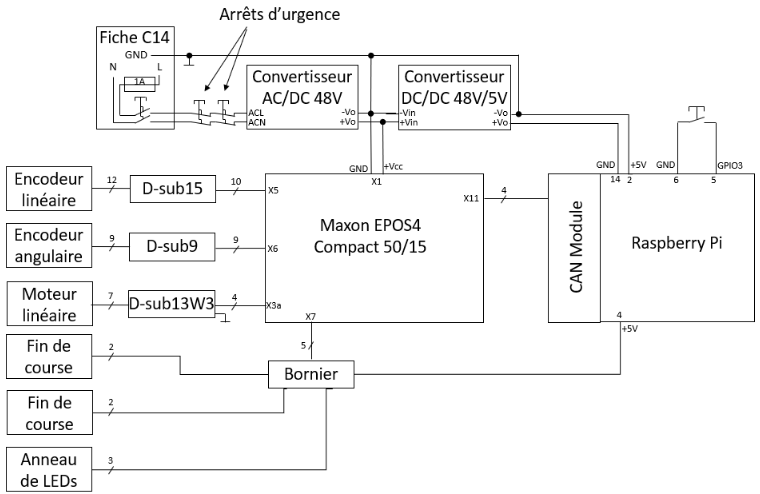
\includegraphics[width = 0.8\textwidth]{assets/figures/SchemaElectrique.svg}
    \caption{Schéma électrique des branchements des éléments du boîtier}
    \label{fig:SchemaElec}
\end{figure}

\subsection{Carte de contrôle}
Les deux encodeurs, l'anneau de LEDs, le moteur et les fins de courses sont tous connectés sur le contrôleur EPOS4 qui est dirigé par la carte
RaspberryPi. Les fins de courses et l'anneau de LEDs passent par un bornier qui regroupe ensuite les fils en un seul câble qui se branche
sur le port d'entrées/sorties digitales X7. Le moteur est branché sur le port X3a prévu à cet effet et les deux encodeurs se branchent sur
le port pour encodeur X5 et senseur X6. Les ports, connecteurs et composants à connecter sont expliqués en détail dans la \textit{datasheet}
du contrôleur EPOS4 de Maxon \cite{Maxon} en annexe C.

\subsection{Carte de commande}

La carte est alimentée en 5V sur les pins 2 (+5V) et 14 (GND) depuis le convertisseur 48V/5V. Un module de communication CAN pour RaspberryPi est
placé sur la carte afin de pouvoir communiquer par CAN avec le contrôleur. Un bouton poussoir branché sur les pins 5 (GPIO3) et 6 (GND) permet de
mettre en veille et de réveiller le système.
